\documentclass{standalone} %tipo de documento "imagens solo".

\usepackage{tikz} %para imagens e gráficos vetoriais

\usepackage{circuitikz} %para desenhar circuitos elétricos

\usepackage{tkz-euclide} %define pontos no plano cartesiano

\usepackage{xcolor} %utilização de cores para estilos específicos 

\begin{document}

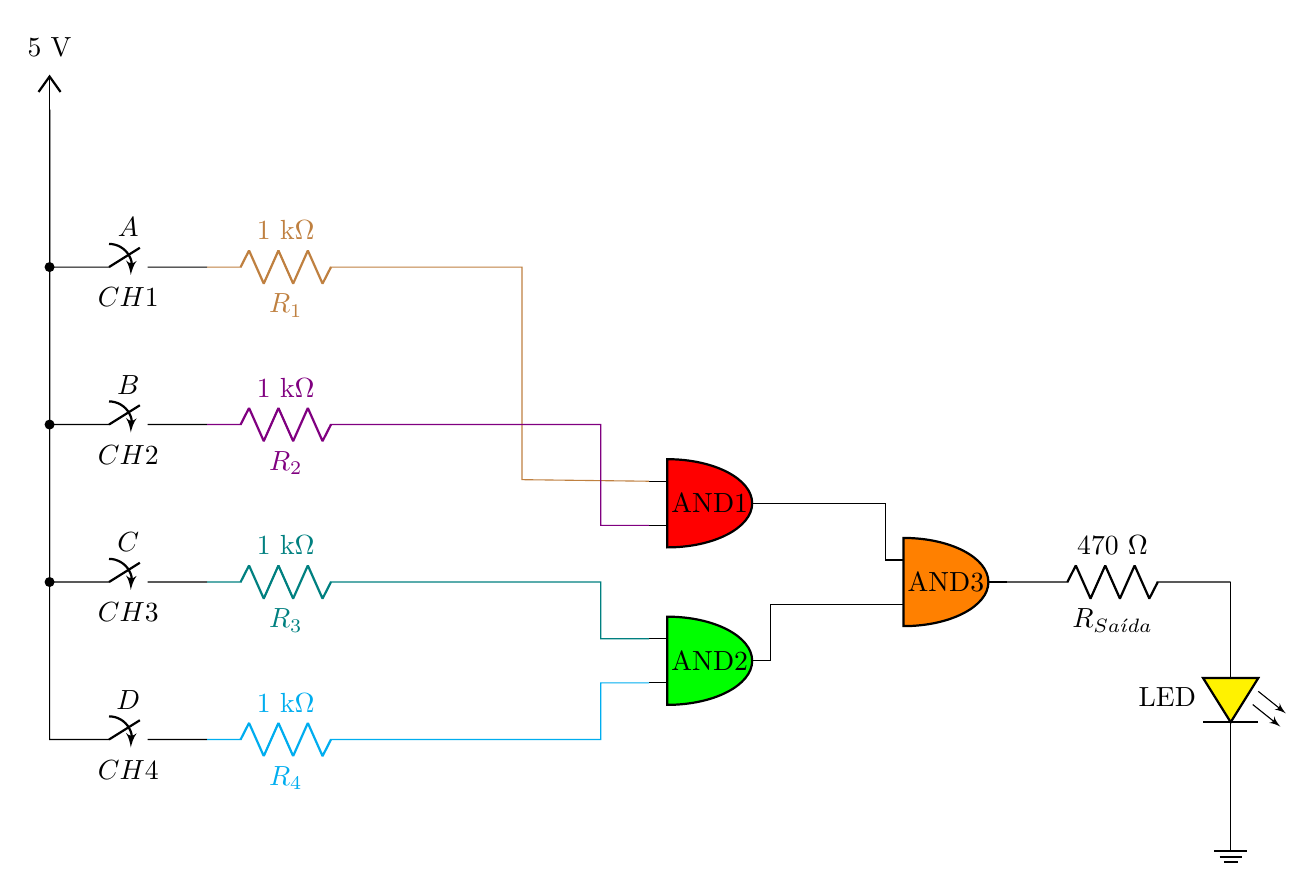
\begin{tikzpicture}[american] %define a tipologia dos componentes do circuito

%----------------------------------------------------
%Desenhar e posicionar todos os elementos
%----------------------------------------------------
\draw[fill=green] (0,0) node[and port](AND2) {AND2}; %desenha uma AND preenchida com a cor verde na posição (0,0)
\draw[fill=red] (0,2) node[and port](AND1) {AND1}; %desenha uma AND preenchida com a cor vermelha na posição (0,2)
\draw[fill=orange] (3,1) node[and port](AND3) {AND3}; %desenha uma AND preenchida com a cor laranja na posição (3,1) 

%----------------------------------------------------
%Desenhar o circuito de entrada
%----------------------------------------------------

%alimentação
\draw (-9,7)node[vcc](vcc){5 V}; %desenha a fonte VDD "simplificada"

%entrada A
\draw (-9,7)--(-9,5) to [closing switch, a=$CH1$, l=$A$, , *-] (-7,5);

%adicionando a cor marrom no desenho onde o segmento do elemento termina em (-5,5), após isso são os três segmentos para chegar até a entrada 1 da primeira porta lógica AND1.
\draw[brown] (-7,5) to [R, a=$R_1$, l=$1$ k$\Omega$] (-5,5)--(-3,5)--(-3,2.3)--(AND1.in 1); %altura da entrada 1 da AND1=(-3,2.3)

%entrada B
\draw (-9,7)--(-9,3) to [closing switch, a=$CH2$, l=$B$, *-] (-7,3);

%adicionando a cor roxo no desenho onde o segmento do elemento termina em (-5,3), após isso são os três segmentos para chegar até a entrada 2 da primeira porta lógica AND1.
\draw[violet] (-7,3) to [R, a=$R_2$, l=$1$ k$\Omega$] (-5,3)--(-2,3)--(-2,1.72)--(AND1.in 2); %altura da entrada 2 da AND1=(-2,1.72)

%entrada C
\draw (-9,7)--(-9,1) to [closing switch, a=$CH3$, l=$C$, , *-] (-7,1);

%adicionando a cor verde-azulado no desenho onde o segmento do elemento termina em (-5,1), após isso são os três segmentos para chegar até a entrada 1 da primeira porta lógica AND2.
\draw[teal] (-7,1) to [R, a=$R_3$, l=$1$ k$\Omega$] (-5,1)--(-2,1)--(-2,0.28)--(AND2.in 1); %altura da entrada 1 da AND2=(-2,0.28)

%entrada D
\draw (-9,7)--(-9,-1) to [closing switch, a=$CH4$, l=$D$] (-7,-1);

%adicionando a cor ciano no desenho onde o segmento do elemento termina em (-5,-1), após isso são os três segmentos para chegar até a entrada 2 da primeira porta lógica AND2.
\draw[cyan] (-7,-1) to [R, a=$R_4$, l=$1$ k$\Omega$] (-5,-1)--(-2,-1)--(-2,-0.28)--(AND2.in 2); %altura da entrada 2 da AND2=(-2,-0.28)


%----------------------------------------------------
%Desenhar o circuito de saída
%----------------------------------------------------
\draw (3,1) to [R, a=$R_{Sa\acute{\imath}da}$, l=$470$ $\Omega$] (6,1);
\draw[fill=yellow] (6,1) to [empty led, a=LED] (6,-2) node[ground](GND){}; %desenha um LED preenchido com a cor amarela na posição (6,1) e conectada o GND ao final do segmento 


%----------------------------------------------------
%Desenhar as conexões dentro do bloco lógico saída da AND1 e saída da AND2
%----------------------------------------------------
\draw (AND1.out) -| (AND3.in 1);
\draw (AND2.out) |- (AND3.in 2);

\end{tikzpicture}


\end{document}
